\documentclass[fleqn]{article}

%\pgfplotsset{compat=1.17}

\usepackage{mathexam}
\usepackage{amsmath}
\usepackage{amsfonts}
\usepackage{graphicx}
\usepackage{wrapfig}
\usepackage{systeme}
\usepackage{microtype}
\usepackage{multirow}
\usepackage{pgfplots}
\usepackage{listings}
\usepackage{tikz}
\usepackage{dsfont} %Numeros reales, naturales...
\usepackage{cancel}
\usepackage[spanish]{babel}

%\graphicspath{{images/}}
\newcommand*{\QED}{\hfill\ensuremath{\square}}

%Estructura de ecuaciones
\setlength{\textwidth}{15cm} \setlength{\oddsidemargin}{5mm}
\setlength{\textheight}{23cm} \setlength{\topmargin}{-1cm}



\author{David García Curbelo}
\title{Curvas y Superficies, Prueba Final (Opción B)}
\date{Grado en Matemáticas, Grupo A}

\pagestyle{empty}


\def\R{\mathds{R}}
\def\Z{\mathds{Z}}
\def\N{\mathds{N}}

\def\sup{$^2$}

\def\next{\quad \Rightarrow \quad}

\begin{document}
    \maketitle
    \setcounter{page}{1}
    \pagestyle{plain}



    \textbf{Ejercicio 1. } \\

    Para poder comparar ambas curvas, primero necesitamos que ambas estén parametrizadas por su arco. Vemos que la curva $\alpha(s)$ dada ya está parametrizada por su arco, 
    lo que implica que el módulo de su vector tangente es uno ($|T_{\alpha}(s)| = |\alpha'(s)| = \sqrt{x'(s)^2 + y'(s)^2} = 1$, y por lo tanto $x'(s)^2 + y'(s)^2 = 1$). 
    Parametricemos a continuación la curva $\gamma$. Vemos que su vector tangente (y respectivamente su módulo) vienen dados por

    $$T_{\gamma}(s) = (x'(s), y'(s), a) \quad \quad \quad \quad |T_{\gamma}(s)| = \sqrt{x'(s)^2 + y'(s)^2 + a^2} = \sqrt{1 + a^2} $$
    Y por lo tanto al parametrizar por el arco obtenemos

    $$t(s) = \int_0^s |T_{\gamma}(s)| du = \int_0^s \sqrt{1 + a^2} du = s\sqrt{1 + a^2} \next s = \frac{t}{\sqrt{1 + a^2}}$$
    Y obtenemos la curvas parametrizadas en la nueva notación 
    $$\alpha(t) = (x(t), y(t), 0) \quad \quad \quad \quad \gamma(t) = \left(x \left(\frac{t}{\sqrt{1 + a^2}}\right), y \left(\frac{t}{\sqrt{1 + a^2}}\right), \frac{a}{\sqrt{1 + a^2}} \right) $$
    
    Sabemos que los aparatos de Frenet de una curva son los vectores tangente, normal y binormal, además de sus funciones curvatura y torsión. Procedamos a calcular cada uno de estos elementos
    para ambas curvas que queremos comparar.

    $$T_{\alpha}(t) = \left( x'(t), y'(t), 0 \right)$$

    $$T_{\gamma}(t) = \left(\frac{1}{\sqrt{1 + a^2}} x'\left(\frac{t}{\sqrt{1 + a^2}}\right), \frac{1}{\sqrt{1 + a^2}} y'\left(\frac{t}{\sqrt{1 + a^2}}\right), \frac{a}{\sqrt{1 + a^2}} \right)$$
    $$ = \frac{1}{\sqrt{1 + a^2}}\left( x'\left(\frac{t}{\sqrt{1 + a^2}}\right), y'\left(\frac{t}{\sqrt{1 + a^2}}\right), a\right) = 
    \frac{1}{\sqrt{1 + a^2}} \left( T_{\alpha}\left(s\right) + a\cdot \vec{e}_3 \right)$$\\

    Para el cálculo del vector normal procedemos primero al cálculo de la derivada y del módulo de los vectores tangentes
    $$T_{\alpha}'(t) = ( x''(t), y''(t), 0) \quad \quad \quad \quad |T_{\alpha}'(t)| = \sqrt{x''(t)^2 + y''(t)^2}$$
    $$ N_{\alpha}(t) = \frac{T_{\alpha}'(t)}{|T_{\alpha}'(t)|} = \frac{1}{\sqrt{x''(t)^2 + y''(t)^2}} ( x''(t), y''(t), 0) $$

    $$T_{\gamma}'(t) = \frac{1}{1 + a^2}\left( x''\left(\frac{t}{\sqrt{1 + a^2}}\right), y''\left(\frac{t}{\sqrt{1 + a^2}}\right), 0\right) \quad \quad \quad 
    |T_{\gamma}'(t)| = \frac{1}{1 + a^2}\sqrt{x''\left(\frac{t}{\sqrt{1 + a^2}}\right)^2 + y''\left(\frac{t}{\sqrt{1 + a^2}}\right)^2}$$
    
    $$ N_{\gamma}(t) = \frac{T_{\gamma}'(t)}{|T_{\gamma}'(t)|} = 
    \frac{1}{\sqrt{x''\left(\frac{t}{\sqrt{1 + a^2}}\right)^2 + y''\left(\frac{t}{\sqrt{1 + a^2}}\right)^2}}\left( x''\left(\frac{t}{\sqrt{1 + a^2}}\right), y''\left(\frac{t}{\sqrt{1 + a^2}}\right), 0\right)
    = N_{\alpha}\left(s\right)$$\\

    El vector binormal viene dado por el producto vectorial de los vectores tangente y normal, luego:

    $$B_{\alpha}(t) = T_{\alpha}(t) \times N_{\alpha}(t)$$

    $$B_{\gamma}(t) = T_{\gamma}(t) \times N_{\gamma}(t) = \left[ \frac{1}{\sqrt{1 + a^2}} \left( T_{\alpha}(s) + a\cdot \vec{e}_3 \right) \right] \times N_{\alpha}(s)
    = \frac{1}{\sqrt{1 + a^2}} \left[ T_{\alpha}(s) \times N_{\alpha}(s) +  \vec{e}_3a \times N_{\alpha}(s) \right] = $$
    $$ = \frac{1}{\sqrt{1 + a^2}} \left[ B_{\alpha}(s) + \frac{a}{|T_{\gamma}'(t)|} (-y''(s), x''(s), 0)\right] = \frac{1}{\sqrt{1 + a^2}} \left[ B_{\alpha}(s) + a\cdot J(\frac{T_{\gamma}'(t)}{|T_{\gamma}'(t)|}) \right] $$
    $$B_{\gamma}(t) = \frac{1}{\sqrt{1 + a^2}} \left[ B_{\alpha}(s) + a\cdot J( N_{\alpha}(s)) \right]$$\\

    Donde $J$ representa un giro de $90$º con respecto al vector $\vec{e}_3$. Procedemos a continuación al cálculo de la torsión y de la curvatura.

    $$k_{\alpha}(t) = \frac{T_{\alpha}'(t)}{N_{\alpha}(t)} = |T_{\alpha}'(t)| = \sqrt{x''(t)^2 + y''(t)^2} $$
    $$k_{\gamma}(t) = \frac{T_{\gamma}'(t)}{N_{\gamma}(t)} = \frac{1}{1 + a^2}\sqrt{x''\left(\frac{t}{\sqrt{1 + a^2}}\right)^2 + y''\left(\frac{t}{\sqrt{1 + a^2}}\right)^2} = \frac{1}{1 + a^2} k_{\alpha}(s) $$

    Para el cálculo de la torsión es necesario el cálculo previo de la derivada del vector binormal.

    $$B_{\gamma}'(t) = \frac{1}{\sqrt{1 + a^2}} \left[ B_{\alpha}'(s) + a\cdot J( N_{\alpha}'(s)) \right] $$

    $$\tau_{\gamma}(t) = \langle N_{\gamma}(t), B_{\gamma}'(t) \rangle = 
    \frac{1}{\sqrt{1 + a^2}} \left[ \langle N_{\alpha}(s), B_{\alpha}'(s) \rangle  + a \langle N_{\alpha}(s), J( N_{\alpha}'(s)) \rangle \right] = $$
    $$= \frac{1}{\sqrt{1 + a^2}} \left[ \tau_{\alpha}(s) + a \langle N_{\alpha}(s), J( N_{\alpha}'(s)) \rangle \right]$$

    Por lo tanto hemos obtenido las siguientes relaciones entre los aparatos de Frenet de ambas curvas (donde $s$ viene dado por $s = \frac{t}{\sqrt{1+a^2}}$):

    $$
    \left[
        \begin{aligned}
            T_{\gamma}(t) &= \frac{1}{\sqrt{1 + a^2}} \left( T_{\alpha}\left(s\right) + a\cdot \vec{e}_3 \right)\\
            N_{\gamma}(t) &= N_{\alpha}\left(s\right)\\
            B_{\gamma}(t) &= \frac{1}{\sqrt{1 + a^2}} \left[ B_{\alpha}(s) + a\cdot J( N_{\alpha}(s)) \right]\\
            k_{\gamma}(t) &= \frac{1}{1 + a^2} k_{\alpha}(s)\\
            \tau_{\gamma}(t) &= \frac{1}{\sqrt{1 + a^2}} \left[ \tau_{\alpha}(s) + a \langle N_{\alpha}(s), J( N_{\alpha}'(s)) \rangle \right]        
        \end{aligned}
    \right]
    $$

    \newpage






















    \textbf{Ejercicio 2. } \\
    
    Estudiemos primero la regularidad de nuestra aplicación dada 
    $$F(s,v) = \alpha(s) + vB(s)$$
    Como sabemos que la curva $\alpha (s)$ tiene curvatura positiva, esto implica que tanto el módulo de su vector tangente como el de su vector normal son no nulos en toda la curva,
    y consecuentemente su vector binormal tampoco, por ser el resultado del producto vectorial de los dos anteriores. Sabiendo esto, estudiar la regularidad de nuestra función $F$ es 
    sencillo, ya que sólo necesitamos comprobar que el Jacobiano asociado tenga rango dos para todo $s\in I$. Para ello consideremos la matriz jacobiana siguiente
    $$
    J(F(s,v)) = 
    \begin{pmatrix}
        \frac{\partial}{\partial s} F(s,v)\\
        \frac{\partial}{\partial v} F(s,v)
    \end{pmatrix}
    =
    \begin{pmatrix}
        \alpha'(s) + vB'(s) \\
        B(s)
    \end{pmatrix}
    =
    \begin{pmatrix}
        T(s) + vB'(s) \\
        B(s)
    \end{pmatrix}
    $$
    Sabemos por definición que la derivada del binormal es proporcional al vector normal de nuestra curva (que lo notaremos por $\xi(s)$), por lo que $T(s) + vB'(s)$ pertenece al plano osculador. Como el vector
    binormal es ortogonal al plano osculador, tenemos que $T(s) + vB'(s)$ y $B(s)$ son dos vectores ortogonales, y por ello el rango de la matriz jacobiana es mayor que 1
    (particularmente 2) y por tanto tenemos que la aplicación $F$ es regular, como queríamos probar.

    Considerando ahora la superficie $S=F(U)$, siendo $U$ un abierto sobre el que $F$ es inyectiva, podemos ver fácilmente que dicha superficie $S$ es una superficie regular por ser 
    grafo de $F(s,v)$. Dicha superficie la podemos parametrizar de la siguiente forma:
    $$
    \begin{aligned}
        X:U \subset \R^2 \longrightarrow X(U) = S \\
        X(s,v) = \alpha(s) + vB(s)
    \end{aligned}
    $$
    De la que podemos obtener una base del plano tangente a la superficie:
    $$X_s = \alpha'(s) + vB'(s) \quad \quad \quad \quad X_v = B(s)$$
    Y por tanto podemos obtener fácilmente el vector normal a la superficie, el cual viene dado por 
    $$N = \frac{X_s \times X_v}{|X_s \times X_v|}$$
    $$X_s \times X_v = \left(\alpha'(s) + vB'(s)\right) \times B(s) = \alpha'(s) \times B(s) + v\left(B'(s) \times B(s)\right) = T(s) \times B(s) + v\lambda \left(\xi(s) \times B(s)\right)
    $$$$=  \lambda v T(s) - \xi(s) , \quad \lambda \in \R$$

    $$\Rightarrow N = \frac{1}{z} \left( \lambda v T(s) - \xi(s) \right), \quad z = |X_s \times X_v|$$

    Para proceder al cálculo de la función curvatura de Gauss y poder clasificar correctamente sus puntos, consideremos la matriz asociada al operador forma,
    la cual sabemos que viene dada por 

    \begin{equation*}
        A =
        \begin{pmatrix}
            a_{11} & a_{12} \\
            a_{21} & a_{22}
        \end{pmatrix}
        = \frac{1}{\langle X_s, X_s \rangle \langle X_v, X_v \rangle - \langle X_s, X_v \rangle ^2}
        \begin{pmatrix}
            \langle X_v, X_v \rangle & - \langle X_s, X_v \rangle \\
            -\langle X_s, X_v \rangle & \langle X_s, X_s \rangle
        \end{pmatrix}
        \begin{pmatrix}
            \langle X_{ss}, N \rangle & \langle X_{sv}, N \rangle \\
            \langle X_{vs}, N \rangle & \langle X_{vv}, N \rangle
        \end{pmatrix}
    \end{equation*}

    Calculando sus elementos obtenemos:

    $$X_{ss} = \alpha''(s) + vB''(s) \quad \quad X_{sv} = B'(s) = X_{vs} \quad \quad X_{vv} = 0$$

    $$\langle X_s, X_s \rangle = |\alpha'(s) + vB'(s)|^2 \quad \quad \quad \langle X_s, X_v \rangle = 0  \quad \quad \quad \langle X_v, X_v \rangle = |B(s)|^2$$

    $$\langle X_{ss}, N \rangle \quad \quad \quad \langle X_{sv}, N \rangle = \langle X_{vs}, N \rangle = \frac{-\tau(s)}{z} \quad \quad \quad \langle X_{vv}, N \rangle = 0$$

    Con lo que resulta la matriz

    $$
        A =
        \frac{1}{\left(|\alpha'(s) + vB'(s)||B(s)|\right)^2}
        \begin{pmatrix}
            |B(s)|^2 & 0 \\
            0 & |\alpha'(s) + vB'(s)|^2
        \end{pmatrix}
        \begin{pmatrix}
            \langle X_{ss}, N \rangle & \frac{-\tau(s)}{z} \\
            \frac{-\tau(s)}{z} & 0
        \end{pmatrix}
    $$

    $$
    A=
    \begin{pmatrix}
        \frac{\langle X_{ss}, N \rangle}{|\alpha'(s) + vB'(s)|^2} & \frac{-\tau(s)}{z\cdot|\alpha'(s) + vB'(s)|^2} \\
        \frac{-\tau(s)}{z\cdot|B(s)|^2} & 0
    \end{pmatrix}
    $$
    Como sabemos que su función curvatura de Gauss viene dada por el determinante de la matriz anterior, vemos fácilmente que dicho determinante resulta
    
    $$det(A) = K = \frac{-\tau(s)^2}{z^2|B(s)|^2|\alpha'(s) + vB'(s)|^2} = - \left(\frac{\tau(s)}{z|B(s)||\alpha'(s) + vB'(s)|}\right)^2$$
    Podemos ver que la curvatura será siempre negativa, a menos que uno de los términos se anule. Como sabemos que la curvatura de la curva $\alpha(s)$ es siempre positiva,
    sabemos que ninguno de los componentes del triedro de Frenet se anula, luego $|B(s)|$ es no nulo. Además, el término $z = |X_s \times X_v|$ tampoco se anula, ya que
    $$X_s \times X_v = \lambda v T(s) - \xi(s)$$ 
    y ambos vectores tangente y normal son ortogonales (linealmente independientes), y por tanto no se anulan. Por último nos falta comprobar $|\alpha'(s) + vB'(s)|\neq 0$,
    pero si consideramos que $B'(s)$ es proporcional al vector normal de la curva, nos encontramos en el mismo caso que el anterior, donde obtenemos
    $$|\alpha'(s) + vB'(s)| = |T(s) + v\lambda \xi(s)|$$
    Y como sabemos que $T$ y $\xi$ son ortogonales, entonces vemos que nunca se cancelan entre sí. Por ello llegamos a la conclusión que la anulación de la curvatura de Gauss viene condicionada
    por la anulación de su torsión, y como sabemos que $\alpha(s)$ tiene curvatura positiva $\forall s \in I$, podemos concluir que dichos puntos donde la torsión toma valor 0 
    serán puntos parabólicos, y cualquier otro punto de la superficie (por haber obtenido curvatura de Gauss negativa) será un punto hiperbólico.

    \newpage


















    \textbf{Ejercicio 3. } \\

    Consideremos para el cálculo de la parametrización que buscamos la recta que pasa por cualquier punto del plano proyectante $xy$ (de la forma $(x,y,0)$) y el punto $(0,0,1)$,
    la cual viene dada por $L = (0,0,1) + \lambda (x,y,-1)$ con $\lambda \in \R$. Calculando el punto de intersección con la esfera unidad obtenemos que 
    dicho punto se representa de la siguiente manera
    
    $$\left(\frac{2x}{x^2 + y^2 + 1}, \frac{2y}{x^2 + y^2 + 1}, \frac{x^2 + y^2 - 1}{x^2 + y^2 + 1}\right) = E^{-1}(x,y) = X(x,y) $$
    Con lo que hemos obtenido la aplicación que buscábamos. Veamos si dicha parametrización cumple alguna de las cuestiones planteadas. Calculemos primero los coeficientes
    de la primera forma fundamental, que nos serán útiles para la resolución del ejercicio.
    
    $$X_x = \left( 2\frac{- x^2 + y^2 + 1}{(x^2 + y^2 + 1)^2}, \frac{ - 4xy}{(x^2 + y^2 + 1)^2}, \frac{4x}{(x^2 + y^2 + 1)^2} \right) $$
    $$X_y = \left( \frac{ - 4xy}{(x^2 + y^2 + 1)^2}, 2\frac{x^2 - y^2 + 1}{(x^2 + y^2 + 1)^2}, \frac{4y}{(x^2 + y^2 + 1)^2} \right) $$

    $$E = \langle X_x,X_x \rangle = 4\frac{(x^2 + y^2)(x^2 + y^2 + 2) + 1}{(x^2 + y^2 + 1)^4} = \langle X_y,X_y \rangle = G; \quad \quad \quad \quad
    F = \langle X_x,X_y \rangle = 0
    $$
    Como $\langle X_x,X_y \rangle = 0$, entonces las familias de curvas coordenadas se cortan ortogonalmente, y por tanto podemos afirmar que la aplicación $X$
    se trata de una proyección ortogonal.

    Para las siguientes dos cuestiones, sabemos bien que una aplicación se dice isoterma si y sólo si se trata de una aplicación conforme. Por definición sabemos que una 
    parametrización se dice isoterma si sus coeficientes de la primera forma fundamental cumplen $E=G$ y $F=0$. Como vimos anteriormente, nuestra parametrización $X(x,y)$
    cumple dicha hipótesis, por lo tanto podemos afirmar que dicha parametrización es isoterma y que, por tanto, se trata de una aplicación conforme.

    \newpage























    \textbf{Ejercicio 4. } \\

    Estudiemos las geodésicas de una superficie de revolución, y veamos posteriormente qué condiciones ha de cumplir la curva perfil para que alguna de 
    dichas geodésicas sea un paralelo de la superficie de revolución. Para ello consideremos la parametrización de cualquier superficie $S$ de revolución,
    que sabemos que viene dada por 
    
    $$X(u,v) = (x(u)\cos(v), x(u) \sin(v), z(u))$$
    $$X_u = (x'(u)\cos(v), x'(u)\sin(v), z'(u)) \quad \quad \quad X_v = (-x(u)\sin(v), x(u)\cos(v), 0 )$$
    para una curva perfil $\alpha$ de la forma $\alpha(u) = (x(u), 0, z(u))$. Sabemos que todas las geodésicas de nuestra superficie $S$ vienen dadas por 
    la solución del siguiente sistema de ecuaciones diferenciales ordinarias de segundo orden

    $$\left\{
    \begin{aligned}
        & u''(t) + \Gamma_{11}^1 (u'(t))^2 + 2\Gamma_{12}^1 u'(t) v'(t) + \Gamma_{22}^1 (v'(t))^2 = 0\\
        & v''(t) + \Gamma_{11}^2 (u'(t))^2 + 2\Gamma_{12}^2 u'(t) v'(t) + \Gamma_{22}^2 (v'(t))^2 = 0
    \end{aligned}
    \right.$$
    donde las geodésicas que buscamos tienen la forma $\beta(u(t), v(t))$, y los elementos $\Gamma_{ij}^k$ son los símbolos de Christoffel. Para calcular dichos
    símbolos nos ayudaremos de la primera forma fundamental, cuyos coeficientes $E, \thinspace F, \thinspace G$ vienen dados por 

    $$E = \langle X_u,X_u \rangle = |\alpha'(u)|^2 = 1 \quad \quad 
    F = \langle X_u,X_v \rangle = 0 \quad \quad 
    G = \langle X_v,X_v \rangle = -x(u)^2 $$
    Y por lo tanto los símbolos de Christoffel vienen dados por la siguiente ecuación matricial.
    $$
    \begin{pmatrix}
        \Gamma_{11}^1 & \Gamma_{12}^1 & \Gamma_{22}^1\\
        \Gamma_{11}^2 & \Gamma_{12}^2 & \Gamma_{22}^2
    \end{pmatrix}
    = \frac{1}{2(EG-F^2)}
    \begin{pmatrix}
        G & -F \\
        -F & E
    \end{pmatrix}
    \begin{pmatrix}
        E_u & E_v & 2F_v - G_u \\
        2F_u - E_v & G_u & G_u
    \end{pmatrix}
    $$

    $$
    \begin{pmatrix}
        \Gamma_{11}^1 & \Gamma_{12}^1 & \Gamma_{22}^1\\
        \Gamma_{11}^2 & \Gamma_{12}^2 & \Gamma_{22}^2
    \end{pmatrix} = 
    \begin{pmatrix}
        0 & 0 & - x(u)x'(u) \\
        0 & \frac{x'(u)}{x(u)} & 0
    \end{pmatrix}
    $$
    Teniendo ya los símbolos de Christoffel, podemos volver al sistema de ecuaciones diferenciales antes planteado, el cual se nos queda de la siguiente forma:
    
    $$\left\{
    \begin{aligned}
        & u''(t) - x(u)x'(u) (v'(t))^2 = 0\\
        & v''(t) + 2\frac{x'(u)}{x(u)} u'(t) v'(t) = 0
    \end{aligned}
    \right.$$

    Ahora, como lo que queremos estudiar es si entre los paralelos de nuestra superficie de revolución hay alguna curva geodésica, tomaremos por tanto un valor $u_0$ 
    constante, y estudiaremos si las curvas de la forma $\beta(t) = X(u_0, v(t))$ son geodésicas. Sustituyendo en nuestro sistema anterior obtenemos

    $$\left\{
    \begin{aligned}
        & x(u_0)x'(u_0) (v'(t))^2 = 0\\
        & v''(t) = 0
    \end{aligned}
    \right.$$
    Como $v(t)$ no puede ser constante (ya que si no estaríamos trabajando con un punto en vez de con una curva), entonces tenemos que $v'(t) \neq 0$ y por tanto deducimos
    que $x'(u_0) = 0$. Del mismo modo, si nuestra curva $\beta(t)$ cumple $x'(u_0) = 0$ (extremo relativo), vemos que la primera ecuación del sistema se satisface trivialmente, y la segunda
    ecuación tiene solución afín. Por ello podemos concluir que existirán paralelos que serán curvas geodésicas siempre la función $x(u)$ tenga un punto crítico en $u_0$,
    ($x'(u_0) = 0$). Esto es, en otras palabras, que la distancia de la generatriz al eje de giro sea un punto crítico. Por ello, vemos que en el caso dado en el enunciado
    en que dicha generatriz es cerrada, podemos afirmar que al menos dos de sus paralelos son curvas geodésicas, dadas por al menos un punto mínimo y un punto máximo de 
    distancia con el eje de giro (que en este caso lo hemos tomado como eje $z$).

    \newpage


























    \textbf{Ejercicio 5. } \\

    La cuestión planteada es cierta. Demostraremos cada una de las implicaciones por separado.\\

    \fbox{$\Rightarrow$} \\

    Partimos de que tenemos una curva $\alpha(t)$ la cual es geodésica del cilindro recto, y que por ello sabemos que su aceleración tangencial es nula. 
    Consideremos por ello la parametrización del cilindro (con curva directriz $\beta(t)=(x(t), y(t))$ parametrizada por el arco), la cual viene dada por 

    $$X(t,v) = (x(t), y(t), v) \quad \quad \quad \quad X_t = (x'(t), y'(t), 0) \quad \quad \quad \quad X_v = (0,0,1)$$
    Y cuyos coeficientes de su primera forma fundamental son los siguientes
 
    $$
    E = \langle X_t,X_t \rangle = |\beta'(t)|^2 = 1 \quad \quad 
    F = \langle X_t,X_v \rangle = 0 \quad \quad 
    G = \langle X_v,X_v \rangle = 1
    $$
    Como podemos comprobar, $E=G$ y $F=0$, por lo que podemos afirmar que dicha parametrización es isoterma, y por tanto es una aplicación conforme. Siendo nuestra parametrización una 
    aplicación conforme, esto implica que estudiar los ángulos que forman dos curvas en la superficie del cilindro equivale al estudio del ángulo que forman sus curvas asociadas en el 
    plano. 

    \begin{wrapfigure}{r}{0.45\textwidth} %this figure will be at the right
        \centering
        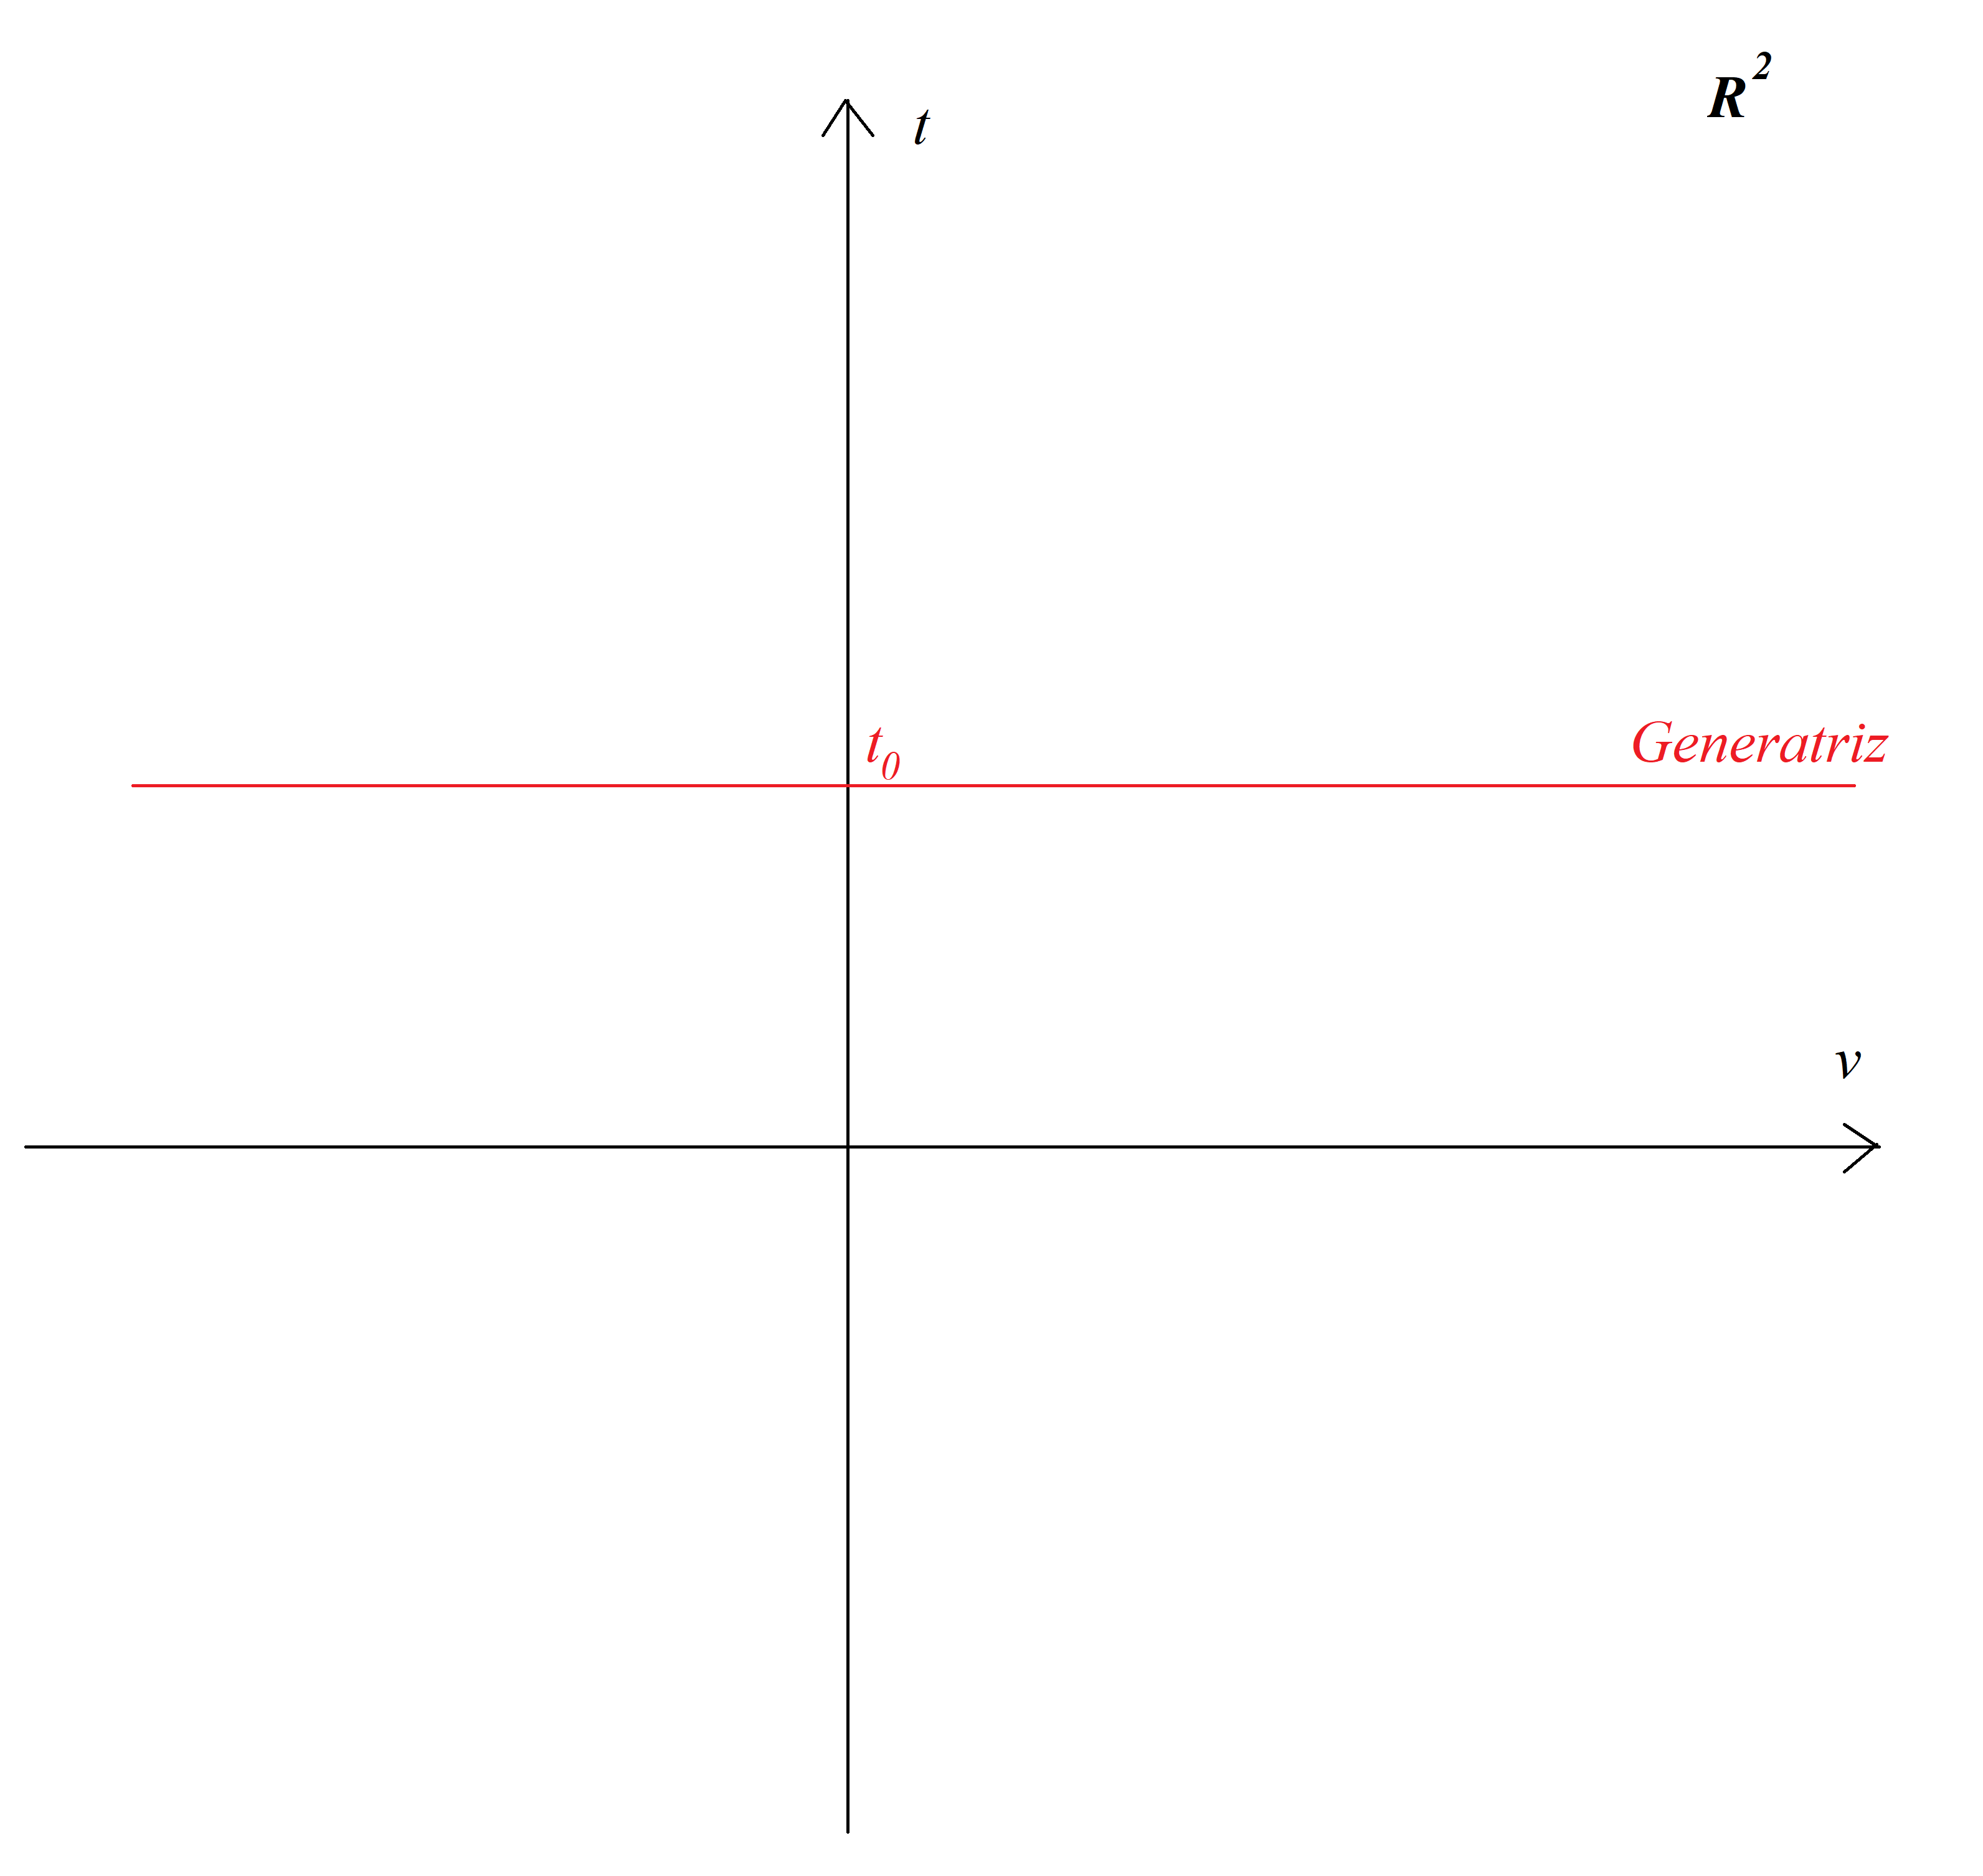
\includegraphics[width=0.45\textwidth]{ejercicio 5.png}
    \end{wrapfigure}

    Por ello consideremos un sistema de coordenadas, donde el eje de absisas (horizontal) lo vamos a asociar con nuestra variable $v$, y el eje de ordenadas con nuestra variable $t$.
    Vemos por tanto en nuestra parametrización, que al considerar cualquier generatriz del cilindro, en el plano equivale a una recta horizontal, cuyo corte con el eje de ordenadas depende de $t_0$ 
    (es decir, depende de cuál de las generatrices hayamos tomado). Como hemos supuesto que nuestra curva $\alpha(t)$ es geodésica, esto implica que su aceleración tangencial es nula,
    y que por tanto su pendiente en el plano va a ser constante (lo cual nos indica que nos encontramos ante una recta afín en el plano). Al ser esto así, vemos que su vector tangente 
    en cada punto va a ser el mismo (ya que es constante), y que por tanto el ángulo $\theta$ que forma con cada una de las generatrices será el mismo. Es decir, que toda geodésica de un cilindro recto
    forma un ángulo constante con las generatrices del cilindro, como queríamos probar.\\

    \fbox{$\Leftarrow$}\\

    Para la demostración del recíproco, el razonamiento es el similar al planteado en la anterior implicación. Partimos de que todas las curvas de un cilindro recto forman ángulo 
    constante con las generatrices, lo cual implica que el módulo de la velocidad es constante. Como ya demostramos antes, la parametrización $X$ es una aplicación conforme, 
    luego podemos considerar que el ángulo que forma la curva con las generatrices en el cilindro debe ser el mismo ángulo que forman en el plano. Como partimos de la hipótesis de que 
    dicho ángulo es constante, esto implica que la pendiente de la curva en el plano ha de ser constante $\forall t_0$. Por ser dicho valor constante,
    vemos que su aceleración en el plano será nula, y consecuentemente en el cilindro su aceleración tangencial valdrá cero, es decir
    $$\frac{D\alpha'(t)}{dt} = 0$$

    \begin{wrapfigure}{l}{0.5\textwidth} %this figure will be at the right
        \centering
        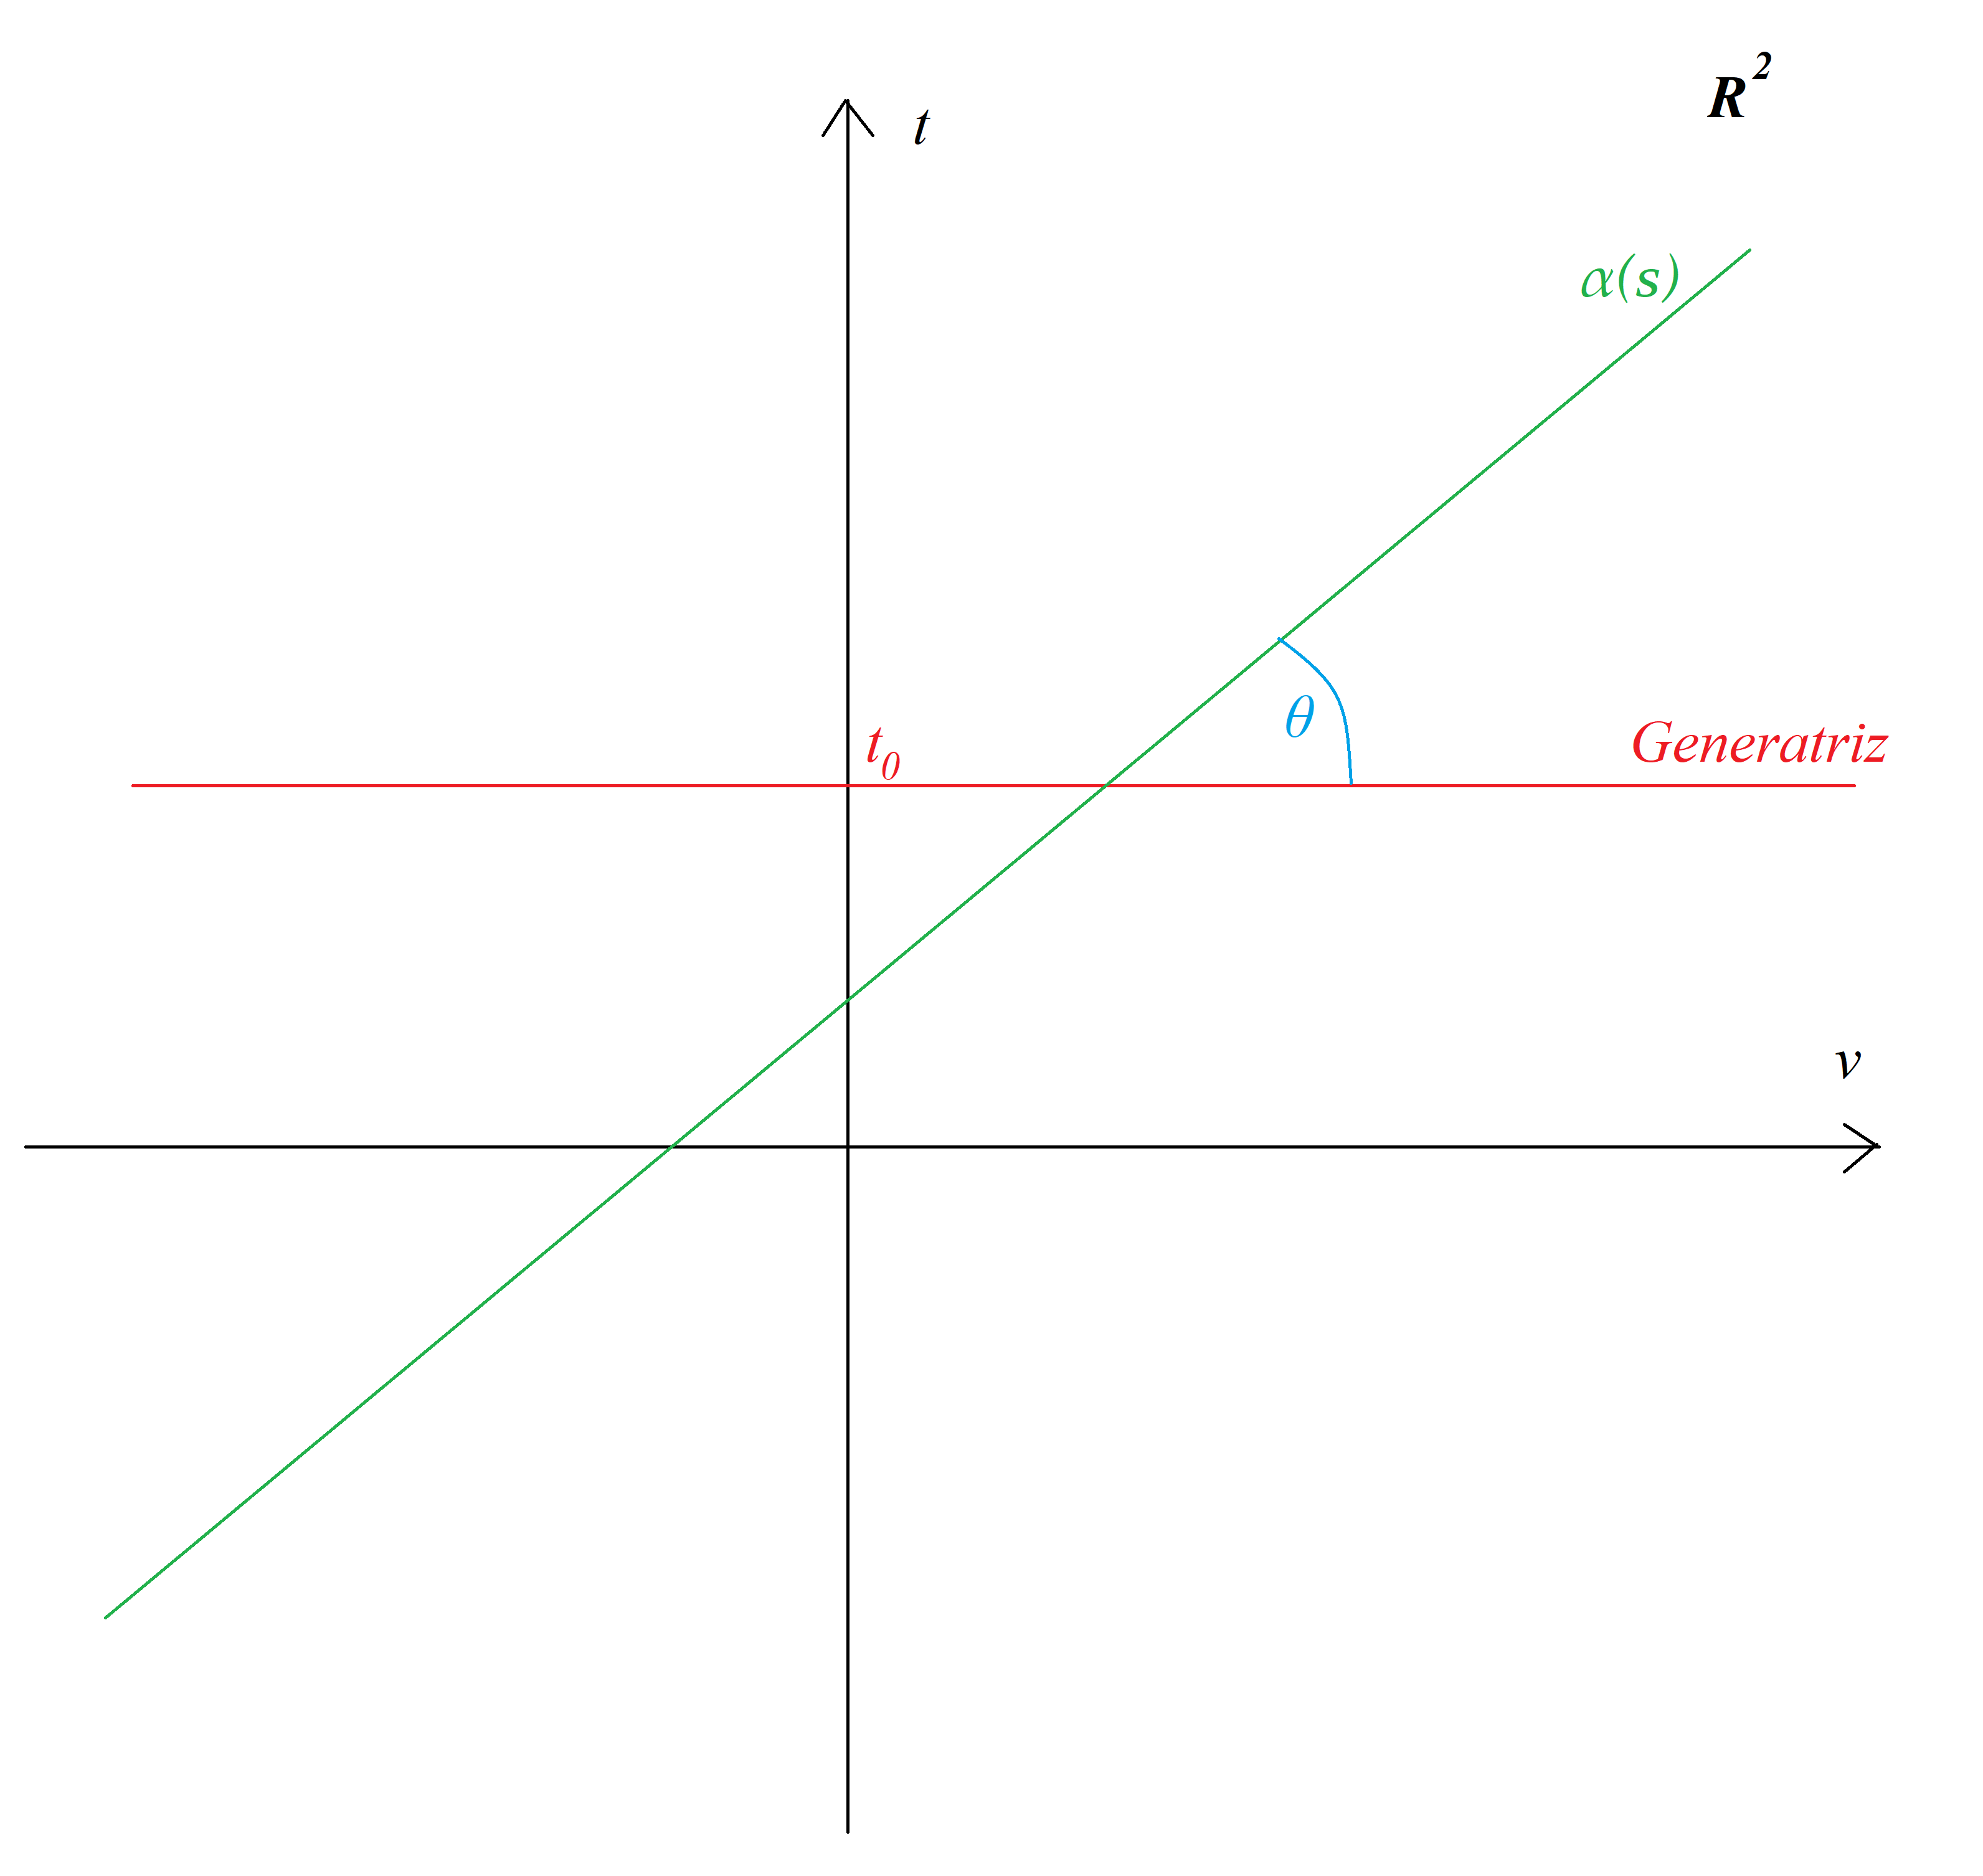
\includegraphics[width=0.5\textwidth]{ejercicio 5 segunda.png}
    \end{wrapfigure}
    
    Como bien sabemos, una curva geodésica es una curva en una superficie cuya aceleración tangencial a la superficie es cero. Por lo que llegamos a la conclusión que 
    toda curva que forme ángulo constante con las generatrices de un cilindro recto es una curva geodésica, como queríamos probar.\\ \\

.\\ \\

.\\ \\

.\\ \\

    \newpage
    











    \textbf{Ejercicio 6. } \\

    Veamos la argumentación para cada una de las dos implicaciones, en las que podemos adelantar que la primera implicación es verdadera y la segunda falsa, 
    demostraciones que desarrollaremos a continuación:
    \begin{enumerate}
        \item \textbf{Congruentes $\Rightarrow$ Globalmente isométricas} \\
                Esta implicación es verdadera. Para demostrarlo consideremos un movimiento rígido $F(p)$ que lleva de una superficie a otra, tal que
                \begin{equation*}
                    \begin{aligned}
                        &F: S_1 \rightarrow S_2\\
                        &F(p) = A\cdot p + \vec{v}
                    \end{aligned}\\
                    \vec{v} \in \R^3\\
                    A \in \mathcal{O}^3 \\
                    p \in S_1
                \end{equation*}
                Estudiando ahora el diferencial de la función, vemos que $DF(p) = A$, que al ser una matriz ortogonal sabemos que su determinante ha de ser $1$ ó $-1$ $\forall p \in S_1$, 
                lo que nos indica que su diferencial en cada punto es una isometría lineal, y por tanto $F$ es una isometría local. Como además sabemos que cualquier movimiento rígido
                es un difeomorfismo global (particularmente nuestro movimiento rígido $F$), concluimos que dicha aplicación es una isometría global.

        \item \textbf{Globalmente isométricas $\Rightarrow$ Congruentes} \\
                Este enunciado es claramente falso. Consideremos una aplicación (parametrización) tal que
                $$F(t, v) = \alpha(t) + v \vec{e}_3 = (\cos (t), \sin (t), v)$$
                donde la curva $\alpha(t) = (\cos (t), \sin (t))$ está parametrizada por su arco, y la aplicación $F(t,v)$ lleva puntos del plano $\R^2$ a puntos del cilindro. Como podemos ver,
                la curva $\alpha(s)$ es una curva simple, por lo que podemos afirmar que nuestra parametrización $F(t,v)$ es una isometría global. Pero sin embargo no es difícil ver que ambas superficies 
                no son congruentes, ya que no existe ningún movimiento rígido que pueda transformar el cilindro en un plano.
    \end{enumerate}


\end{document}